\documentclass[12pt]{article}

\usepackage[spanish]{babel}
\usepackage[none]{hyphenat}
\usepackage[left=1.5cm, right=1.5cm, top = 2cm, bottom=2.5cm]{geometry}
\usepackage{parskip}
\usepackage[export]{adjustbox}
\usepackage{enumitem}[shortlabels]
\usepackage{listings} 
\usepackage{color}
\usepackage{fancyhdr}
\usepackage{graphicx}
\usepackage{caption} 
% \usepackage{subcaption}
% \usepackage{wrapfig}
% \usepackage{longtable}
% \usepackage{multirow, makecell}
% \usepackage{amsmath} 
\usepackage[hidelinks]{hyperref}
\usepackage{csquotes}

\newcommand{\linejump}{\hfill \break}
\renewcommand{\thefootnote}{\fnsymbol{footnote}}
% \newcommand{\unit}[1]{\ensuremath{\, \mathrm{#1}}}

\definecolor{dkgreen}{rgb}{0,0.6,0}
\definecolor{gray}{rgb}{0.5,0.5,0.5}
\definecolor{mauve}{rgb}{0.58,0,0.82}
\lstset{
  language=Java,
  aboveskip=3mm,
  belowskip=3mm,
  showstringspaces=false,
  columns=flexible,
  basicstyle={\scriptsize\ttfamily},
  numbers=none,
  numberstyle=\tiny\color{gray},
  keywordstyle=\color{blue},
  commentstyle=\color{dkgreen},
  stringstyle=\color{mauve},
  breaklines=true,
  breakatwhitespace=true,
  tabsize=2
}

\sloppy
\setlength{\parindent}{0cm}
\setlength{\columnsep}{0.5cm}
\decimalpoint
\graphicspath{{img/}}

\hypersetup{colorlinks=true, urlcolor=blue, citecolor=blue}
\urlstyle{same}

\pagestyle{fancyplain}
\fancyhf{}
\fancyhead[L]{\scriptsize 
  Universidad Nacional Autónoma de México \\
  Laboratorio de Programación Orientada a Objetos \\
  M.C. Leonardo Ledesma Dominguez
}
\fancyhead[R]{\thepage}


\begin{document}
  \begin{center}
    Acosta Porcayo Alan Omar, Gutiérrez Grimaldo Alejandro, Medina Villa Samuel

    \LARGE \textbf{Tarea 4. Herencia y Polimorfismo}
  \end{center}

  \linejump
  \begin{enumerate}[label = \arabic{enumi}]
    \item Investigue y expliqué los tipos de diagrama UML estático.
    \begin{enumerate}[label=\arabic{enumi}.\arabic{enumii}]
      \item \textbf{Diagrama de clases:} Este diagrama se utiliza para representar los elementos que componen un sistema de información desde el punto de vista estático. Esta orientado al modelo de programación orientado a objetos.
      
      En este diagrama se definen las clases que se utilizaran cuando se pase a la fase de construcción.
      
      Esta formado por clases, relaciones e interfaces.
      
      Para encontrar clases sobre un enunciado, sobre una idea o, en general, sobre un tema concreto es buscar los sustantivos que aparecen.

      \begin{figure*}[ht]
        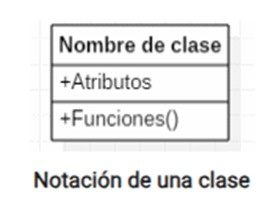
\includegraphics[width = 0.25\textwidth, center]{clase.jpg}
      \end{figure*}
      
      Las relaciones identifican dependencia, esta puede ser entre dos o mas clases. Las relaciones se representan con una línea que une las clases, depende de cada tipo de relación.

      Las interfaces declaran una serie de atributos y métodos, como son declaraciones no pueden ser instancias.

      \begin{figure*}[ht]
        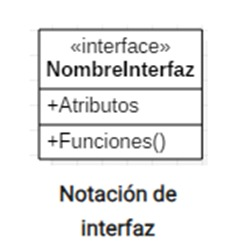
\includegraphics[width = 0.25\textwidth, center]{interface.jpg}
      \end{figure*}

      \item \textbf{Diagrama de objetos:} Los diagramas de objetos muestran un instante en el sistema y las relaciones entre las distintas instancias. 
      
      Estos diagramas se utilizan para modelar los elementos que están presentes en el diagrama de clases. Un diagrama de objetos se puede instanciar como un diagrama de clases.
      
      Los elementos que componen a este diagrama son los objetos, atributos y vínculos.
      
      Los vínculos son asociaciones entre dos objetos, se representan con los mismos elementos que en el diagrama de clases.

      \begin{figure*}[ht]
        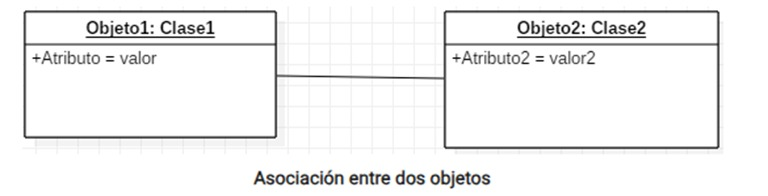
\includegraphics[width = 0.75\textwidth, center]{objeto.jpg}
      \end{figure*}
      
      \item \textbf{Diagrama de componentes:} Los diagramas de componentes representan las relaciones entre los elementos individuales del sistema, pueden ilustrar aspectos de modelado lógico y físico. Los componentes son autocontenidos y encapsulan estructuras de cualquier grado de complejidad.
      
      El diagrama de componentes esta conformado por interfaz, componente y puerto. Este ultimo es un punto de interacción entre un clasificador y un entorno externo. Agrupa un conjunto semánticamente cohesivo de interfaces proporcionadas y requeridas.

      \begin{figure*}[ht]
        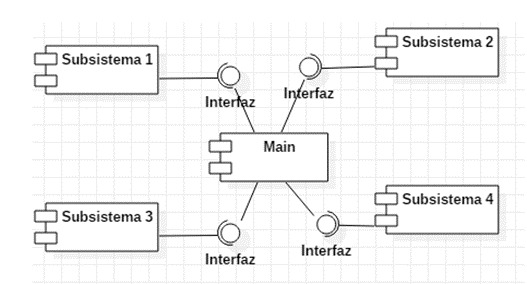
\includegraphics[width = 0.5\textwidth, center]{componente.jpg}
      \end{figure*}
      
      \item \textbf{Diagrama de paquetes:} Este diagrama es utilizado para definir los distintos paquetes a nivel lógico. Su principal objetivo es maximizar la cohesión y minimizar el acoplamiento.
      
      Está conformado por dos elementos: los paquetes y las dependencias.
      Un paquete es un conjunto de elementos. En concreto puede ser un conjunto de clases, casos de uso, componentes u otros paquetes. No obstante, lo más común es que incluya otros paquetes.

      \begin{figure*}[ht]
        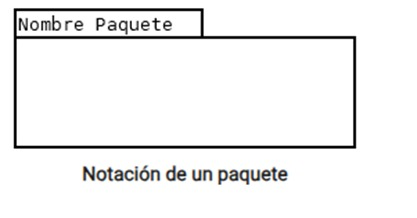
\includegraphics[width = 0.4\textwidth, center]{paquete1.jpg}
      \end{figure*}

      Una dependencia entre paquetes representa que un paquete necesita de los elementos de otro paquete para poder funcionar con normalidad.

      \begin{figure*}[ht]
        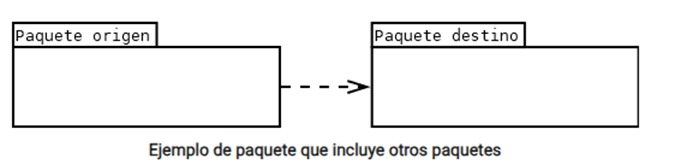
\includegraphics[width = 0.7\textwidth, center]{paquete2.jpg}
      \end{figure*}
    \end{enumerate}

    \linejump
    \item Investigué y expliqué los tipos de diagrama UML dinámico.
    \begin{enumerate}[label=\arabic{enumi}.\arabic{enumii}]
      \item \textbf{Diagrama de actividades:} Son utilizados para representar la forma en la que un sistema hace una implementación.
      
      También son utilizados para modelar el flujo de trabajo entre actividades o/y entre subsistemas. La actividad es una conducta parametrizada representada como flujo coordinado de acciones.  Las actividades pueden formar jerarquías de invocación invocando otras actividades y en última instancia resolviendo acciones individuales. 
      
      \begin{figure*}[ht]
        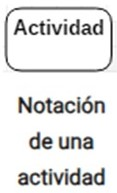
\includegraphics[width = 0.1\textwidth, center]{actividad.jpg}
      \end{figure*}

      \item \textbf{Diagrama de casos de uso:} Representa la forma en como un Cliente (Actor) opera con el sistema en desarrollo, además de la forma, tipo y orden en como los elementos interactúan (operaciones o casos de uso). Un diagrama de casos de uso consta de los siguientes elementos: actor, casos de uso, relaciones de uso, herencia y comunicación. Un Actor es un rol que un usuario juega con respecto al sistema.
      
      Un caso de uso representa una funcionalidad o una unidad de trabajo específica que el sistema debe realizar en respuesta a una solicitud de un actor. Los casos de uso describen cómo el sistema reacciona a una acción del usuario o de otro actor.

      \begin{figure*}[ht]
        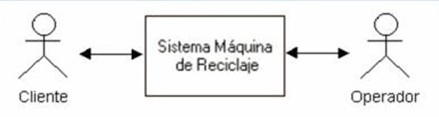
\includegraphics[width = 0.5\textwidth, center]{uso.jpg}
      \end{figure*}
      
      \item \textbf{Diagrama de estados:} Es usado para especificar el comportamiento de una parte del sistema diseñado a través de transiciones de estados finitos.  El comportamiento se modela utilizando una serie de nodos que representan estados y que están conectados a través de las llamadas transiciones.
      
      El estado modela una situación durante la cual se cumple alguna condición invariante (generalmente implícita). Esta situación invariante puede representar una situación estática tal como un objeto que espera que ocurra algún evento externo o cualquier otra situación.
      
      Tenemos diferentes tipos de estados: simple, compuesto y de submáquina.
      
      El diagrama de estados está formado por tres elementos: estados, pseudoestados y transiciones.
      
      \begin{figure*}[ht]
        
\includegraphics[width = 0.1\textwidth, center]{estados.jpg}
      \end{figure*}

      \item \textbf{Diagrama de interacción:} Es una representación gráfica que se utiliza para visualizar y modelar cómo interactúan los objetos en un sistema durante un proceso o escenario específico. Se centran en mostrar la comunicación y la colaboración entre los objetos y las clases que participan en una secuencia de acciones.
      
      Existen dos tipos principales de diagramas de interacción: los diagramas de secuencia y los diagramas de colaboración. 
      
      Los diagramas de secuencia son particularmente útiles para representar la lógica de flujo de un proceso o la ejecución de un caso de uso en un sistema. Los diagramas de colaboración se utilizan para mostrar las relaciones y las interacciones entre objetos en un sistema, pero no se centran en la secuencia temporal como lo hacen los diagramas de secuencia. En su lugar, muestran cómo los objetos se comunican entre sí, incluyendo los mensajes que se envían y las asociaciones entre los objetos.

      \begin{figure*}[ht]
        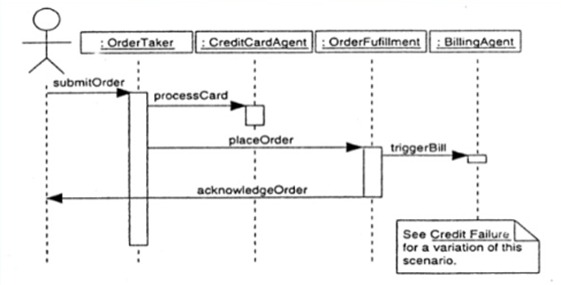
\includegraphics[width = 0.6\textwidth, center]{interaccion.jpg}
      \end{figure*}
      
      \item \textbf{Diagrama de secuencia:} Se utilizan para visualizar y modelar la interacción entre objetos en un sistema a lo largo del tiempo. Estos diagramas representan la secuencia de mensajes que se intercambian entre objetos en un escenario específico o durante la ejecución de un caso de uso en un sistema. 
      
      Algunos elementos clave de este diagrama son los objetos, mensajes, activaciones y notas.
      
      Son herramientas valiosas para comprender y modelar el comportamiento dinámico de un sistema y son ampliamente utilizados durante la fase de análisis y diseño en el desarrollo de software.

      \begin{figure*}[ht]
        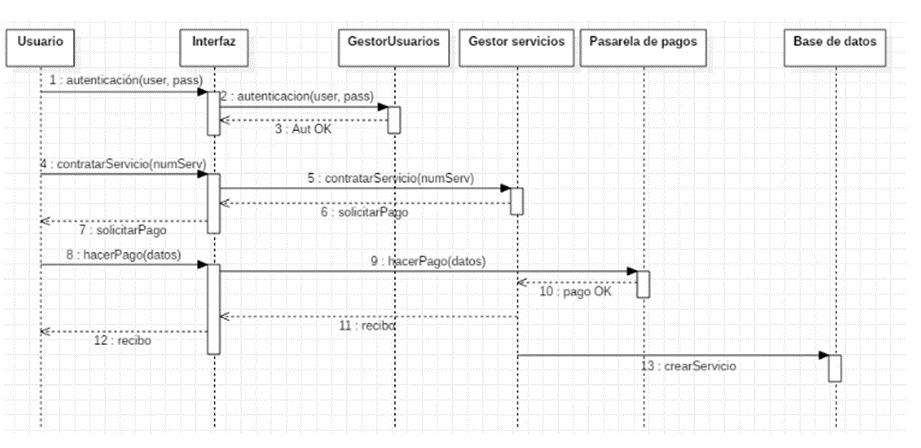
\includegraphics[width = 0.75\textwidth, center]{secuencia.jpg}
      \end{figure*}
      
      \item \textbf{Diagrama de tiempos:} Se emplea para representar el funcionamiento del sistema, con un enfoque particular en la dimensión temporal. Los diagramas temporales se concentran en las variaciones que ocurren tanto dentro como entre las líneas de vida a lo largo de un eje temporal secuencial. Estos diagramas sirven para detallar cómo se comportan los componentes individuales y cómo interactúan entre sí, poniendo énfasis en la cronología de los eventos que provocan cambios en las condiciones de las líneas de vida.
      
      Este diagrama incluye los siguientes elementos: Líneas de vida, Estados, Restricciones de duración y Restricciones de tiempo.
      
      La línea de vida representa a un único participante en la interacción, a pesar de que las partes y las características estructurales puedan tener una multiplicidad mayor que 1.
      
      El diagrama de tiempo tiene la capacidad de mostrar los estados del clasificador o atributo participante, además de condiciones comprobables, como valores discretos de atributos.
      
      La restricción de duración es una limitación temporal que se refiere a un intervalo de duración específico. Este intervalo de duración se utiliza para evaluar si se cumple la restricción en cuestión.
      
      La restricción de tiempo es otra restricción de intervalo, pero en este caso, se relaciona con un período temporal particular.
      
      \begin{figure*}[ht]
        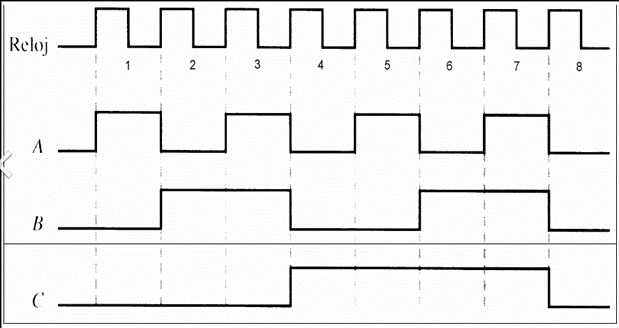
\includegraphics[width = 0.6\textwidth, center]{tiempos.jpg}
      \end{figure*}
    \end{enumerate}

    \newpage \linejump
    \item Programe la simulación de batallas de Transformers
    
    \textbf{Descripción:} 
    \begin{itemize}
      \item Cada transformer tiene su nombre y su raza, un mundo de origen, así como un valor de resistencia, y de uno a dos ataques especiales.
      \item Los ataques / defensas especiales disminuyen de 5 a 10 puntos la resistencia del contrincante o detienen los golpes especiales o básicos de otro contrincante respectivamente. Los ataques especiales son gracias al uso de armas que pueden tener los Transformers.
      \item Las armas tienen un nombre y tipo (defensa o ataque), y en caso de ser de ataque el valor de uso.
      \item Todos tienen ataques básicos: golpe alto 2 puntos y patada 3 puntos.
      \item Además, cada raza tiene un líder y es posible la fusión de dos o mas transformer para hacer uno más grande, dando como resultado la multiplicación de sus resistencias. A esta fusión se les llaman MEGA TRANSFORMER y pueden usar cualquier arma de los transformes que conforman la fusión.
      \item Es posible formar alianzas entre diferentes razas.
      \item Existe el artefacto especial, la matriz de liderazgo que sólo puede ser usada por un líder, al usarla el líder recupera su resistencia inicial y sus golpes especiales aumentan el doble de daño.
    \end{itemize}

    \textbf{Programación}
    \begin{itemize}
      \item Simule una batalla entre dos bandos rivales, cada bando puede estar conformado por una raza o varias. Considere el uso de \textit{ArrayList} para formar los bandos.
      \item Utilice el concepto de Herencia para modelar los tipos de raza de transformer, considere la clase base Transformer y como clases derivadas los tipos de razas.
      \item Considere el uso de una interfaz para modelar MEGA TRANSFORMERS, cabe mencionar que solo algunas razas se pueden fusionar como el caso de los maximals o predacons.
      \item Considere el uso de una clase abstracta para modelar las diferentes armas y tipos de defensa y ataque.
      \item Realice una batalla síncrona (es decir en orden) considerando números aleatorios para simular la batalla:
      \begin{itemize}
        \item Dos números aleatorios entre los índices del \textit{ArrayList} para ver quien ataca y conta quien lanza el ataque del otro bando (del otro \textit{ArrayList}).

        bandoA[i] $\Longrightarrow$ bandoB[j]

        \item Dos números aleatorios, uno en ataque y otro en defensa, en un rango de 1 al 100:
        \begin{itemize}
          \item En ataque: 60 números sean para ataques básicos, 35 números para uso de armas especiales y 5 números especiales (indican el combo de tres golpes básicos)
          \item En defensa: sólo 10 números indican uso de armas especiales de defensa y dos números especiales que son unidades energón que ayudan a reducir el golpe del rival a la mitad. Los 88 números restantes no hacen nada.
        \end{itemize}
      \end{itemize}

      \item Cuando un transformer de cualquier bando tiene menos de la mitad de su resistencia vital, ya no puede continuar seguir peleando y queda derrotado.
      \item Para el jugador líder considere su instanciamiento realizando un upcasting de la superclase con la subclase. Además, utilice downcasting para que la matriz de liderazgo sea un Arma de ataque, pero con las bondades de la superclase y con el método constructor y métodos de la subclase (Arma de ataque).
      \item Use la composición de objetos para simular toda la batalla, y utilice un método estático privado de la superclase Transformer, cuyo método revise en cada momento de la batalla que:
      \begin{itemize}
        \item Haya al menos un derrotado en cualquier bando
        \item Y que todos los jugadores tengan al menos $75\%$ de su resistencia original.
        \item Dicho método solo es invocado por un líderTransformer.
      \end{itemize}
      De ser así otorgue la matriz de liderazgo de manera aleatoria a cualquier bando.

      \item Empaquete el programa realizado de la siguiente manera:
      \begin{itemize}
        \item src/
        \begin{itemize}
          \item battle
          \begin{itemize}
            \item Todos los programas Java
          \end{itemize}
          \item Battle.java (programa que tiene la función \textit{main})
        \end{itemize}
      \end{itemize}

      \item Considere el uso de variables privadas así como sus \textit{getters} \& \textit{setters}.
      \item Aplique el polimorfismo estático y dinámico al menos una vez.Y haga uso al menos una vez del operador \textit{instanceof}.
      \item Al finalizar el programa deberá indicar el bando ganador y el estado de todos los jugadores participantes usando el método \textit{toString}.
    \end{itemize}

    \textbf{Clase \textit{Transformer}}
    \begin{lstlisting}
package src.battle;

import java.util.ArrayList;
import java.util.Random;

public class Transformer implements MegaTransformers {
  private String name;
  private String race;
  private String homePlanet;
  private int enduranceInitial; 
  private int endurance; 
  private ArrayList<Weapons> weapons = new ArrayList<Weapons>();
  private boolean defeated = false;
  private boolean mol = false;

  // Setters
  public void setName(String name) {
    this.name = name;
  }

  public void setRace(String race) {
    this.race = race;
  }

  public void setHomePlanet(String homePlanet) {
    this.homePlanet = homePlanet;
  }

  public void setEnduranceInitial(int enduranceInitial) {
    this.enduranceInitial = enduranceInitial;
  }

  public void setEndurance(int endurance) {
    this.endurance = endurance;
  }

  public void setWeapon(Weapons weapon) {
    this.weapons.add(weapon);
  }

  public void setWeapons(ArrayList<Weapons> weapons) {
    this.weapons = weapons;
  }

  public void setState(boolean defeated) {
    this.defeated = defeated;
  }

  public void setMlf(boolean mol) {
    this.mol = mol;
  }

  // Getters
  public String getName() {
    return this.name;
  }

  public String getRace() {
    return this.race;
  }

  public String getHomePlanet() {
    return this.homePlanet;
  }

  public int getEnduranceInitial() {
    return this.enduranceInitial;
  }

  public int getEndurance() {
    return this.endurance;
  }

  public ArrayList<Weapons> getWeapons() {
    return this.weapons;
  }

  public boolean isDefeated() {
    return this.defeated;
  }

  public boolean getMlf() {
    return this.mol;
  }

  // Methods
  public void getHit(int damage) {
    this.endurance -= damage;
  }

  public int basicAttack() {
    Random rand = new Random();
    int r = rand.nextInt(2);

    if (r == 0) 
      return 8;
    else 
      return 12;
  }

  public void attack(Transformer enemy, ArrayList<Transformer> b1, ArrayList<Transformer> b2) {
    Random random = new Random();
    int rAtk   = random.nextInt(100) + 1;
    int rDef = random.nextInt(100) + 1;
    int damageCount = 0;
    int defenseCount = 0;

    if (rAtk   <= 60) {
      damageCount = this.basicAttack();
      System.out.println(this.getName() + " usa ataque basico");
    } else if (rAtk <= 95) {
      ArrayList<AtkWeapons> atkOptions = new ArrayList<AtkWeapons>();

      for (Weapons i: this.getWeapons()) {
        if (i instanceof AtkWeapons)
          atkOptions.add((AtkWeapons) i);
      }

      int r = random.nextInt(atkOptions.size());
      damageCount = atkOptions.get(r).getDamage();
      System.out.println(this.getName() + " usa " + atkOptions.get(r).getName());
    } else {
      System.out.println(this.getName() + " usa combo de 3 golpes basicos");
      for (int i = 0; i < 3; i ++)
        damageCount += this.basicAttack();
    }

    if (rDef <= 10) {
      ArrayList<DefWeapons> defOptions = new ArrayList<DefWeapons>();

      for (Weapons i: enemy.getWeapons()) {
        if (i instanceof DefWeapons) 
          defOptions.add((DefWeapons) i);
      }
      
      if (defOptions.size() == 0) 
        System.out.println(enemy.getName() + " no tiene armas de defensa");
      else {
        int r = random.nextInt(defOptions.size());
        defenseCount = defOptions.get(r).getDefense();
        System.out.println(enemy.getName() + " usa " + defOptions.get(r).getName());
      }
    } else if (rDef <= 12) {
      defenseCount = damageCount / 2;
      System.out.println(enemy.getName() + " usa unidades de energon");
    } else 
        System.out.println(enemy.getName() + " no se defiende");

    System.out.print(this.getName() + " ataca a " + enemy.getName() + " con " + damageCount + " de danio ");
    System.out.println("y " + enemy.getName() + " se defiende con " + defenseCount + " de defensa");
    if (damageCount - defenseCount > 0)
      enemy.getHit(damageCount - defenseCount);
    System.out.println(enemy.getName() + " queda con " + enemy.getEndurance() + " de resistencia");

    giveMol(b1, b2);
  }

  private static void giveMol(ArrayList<Transformer> b1, ArrayList<Transformer> b2) {
    // Se cambiaron las condiciones para que la matriz se use mas seguido
    boolean defeated1 = false;
    boolean defeated2 = false;
    
    // No da la matriz si ambos lideres estan derrotados
    if (b1.get(0).isDefeated() && b2.get(0).isDefeated())
      return;    

    // No da la matriz si alguno de los dos transformers ya la uso
    if (b1.get(0).getMlf() || b2.get(0).getMlf())
      return;

    // No da la matriz si alguno de los dos lideres tiene mas de 75% de resistencia
    if (b1.get(0).getEndurance() > b1.get(0).getEnduranceInitial()*0.75)
      return;
    
    if (b2.get(0).getEndurance() > b2.get(0).getEnduranceInitial()*0.75)
      return;

    // La da si cada equipo tiene al menos un transformer derrotado
    for (Transformer t : b1) {
      if (t.isDefeated())
        defeated1 = true;
    }
    
    for (Transformer t : b2) {
      if (t.isDefeated())
        defeated2 = true;
    }

    if (!defeated1 || !defeated2)
      return;
        
    Weapons mol = new AtkWeapons("Matriz de Liderazgo");
    if (b1.get(0).isDefeated()) {
      b2.get(0).setMlf(true);
      b2.get(0).useMol();
      System.out.println(b2.get(0).getName() + " obtiene " + mol.getName() + " y la usa");
    } else if (b2.get(0).isDefeated()) {
      b1.get(0).setMlf(true);
      b1.get(0).useMol();
      System.out.println(b1.get(0).getName() + " obtiene " + mol.getName() + " y la usa"); 
    } else {
      Random rand = new Random();
      int n = rand.nextInt(2);

      if (n == 0) {
        b1.get(0).setMlf(true);
        b1.get(0).useMol();
        System.out.println(b1.get(0).getName() + " obtiene " + mol.getName() + " y la usa"); 
      } else {
        b2.get(0).setMlf(true);
        b2.get(0).useMol();
        System.out.println(b2.get(0).getName() + " obtiene " + mol.getName() + " y la usa");
      }
    }
  }

  private void useMol() {
    this.setEndurance(enduranceInitial);
    for (Weapons w : this.getWeapons()) {
      if (w instanceof AtkWeapons) {
        AtkWeapons a = (AtkWeapons) w;
        a.setDamage(a.getDamage() * 2);
      }
    }
  }

  public boolean teamCanFusion(ArrayList<Transformer> b) {
    int count = 0;

    for (Transformer t : b) {
      if (t instanceof Maximal)
        count++;
      
      if (t instanceof Predacon)
        count++;
    }

    if (count >= 2)
      return true;
    else 
      return false;
  }

  public boolean canFusion() {
    return this instanceof Maximal || this instanceof Predacon;
  }

  public void fusion(ArrayList<Transformer> b, int i, int j) {
    System.out.println(b.get(i).getName() + " y " + b.get(j).getName() + " se fusionan en un MegaTransformer");

    String name = b.get(i).getName() + " y " + b.get(j).getName();
    String race = "MegaTransformer";
    int enduranceInitial = b.get(i).getEnduranceInitial() + b.get(j).getEnduranceInitial();
    int endurance = b.get(i).getEndurance() + b.get(j).getEndurance();
    ArrayList<Weapons> weapons = new ArrayList<Weapons>();
    
    for (Weapons w : b.get(i).getWeapons())
      weapons.add(w);

    for (Weapons w : b.get(j).getWeapons())
      weapons.add(w);

    Transformer b1 = b.get(i);
    Transformer b2 = b.get(j);

    b.remove(b1);
    b.remove(b2);

    //Constructor
    Maximal t = new Maximal();
    t.setName(name);
    t.setRace(race);
    t.setHomePlanet("Cybertron");
    t.setEnduranceInitial(enduranceInitial);
    t.setEndurance(endurance);
    t.setWeapons(weapons);
    
    b.add(t);
  }

  public String toString() {
    StringBuilder s = new StringBuilder();

    s.append("Nombre: " + this.name);
    s.append(", Raza: " + this.race);
    s.append(", Mundo de origen: " + this.homePlanet);
    s.append(", Resistencia: " + this.endurance);
    s.append(", Armas: ");
    for (Weapons w : this.weapons)
      s.append(w.getName() + ", ");

    return s.toString();
  }
}    
    \end{lstlisting}

    \textbf{Clase \textit{Autobot}}
    \begin{lstlisting}
package src.battle;

import java.util.ArrayList;

public class Autobot extends Transformer{
  public Autobot(String name, int enduranceInitial , int endurance, ArrayList<Weapons> weapons) {
    setName(name);
    setRace("Autobot");
    setHomePlanet("Cybertron");
    setEnduranceInitial(enduranceInitial);
    setEndurance(endurance);
    setWeapons(weapons);
  }
}    
    \end{lstlisting}
    
    \textbf{Clase \textit{Decepticon}}
    \begin{lstlisting}
package src.battle;

import java.util.ArrayList;

public class Decepticon extends Transformer{
  public Decepticon(String name, int enduranceInitial, int endurance, ArrayList<Weapons> weapons) {
    setName(name);
    setRace("Decepticon");
    setHomePlanet("Cybertron");
    setEnduranceInitial(enduranceInitial);
    setEndurance(endurance);
    setWeapons(weapons);
  }
}    
    \end{lstlisting}

    \textbf{Clase \textit{Maximal}} 
    \begin{lstlisting}
package src.battle;

import java.util.ArrayList;

public class Maximal extends Transformer{
  public Maximal (String name, int enduranceInitial, int endurance, ArrayList<Weapons> weapons) {
    setName(name);
    setRace("Maximal");
    setHomePlanet("Cybertron");
    setEnduranceInitial(enduranceInitial);
    setEndurance(endurance);
    setWeapons(weapons);
  }

  public Maximal () {}
}
    \end{lstlisting}

    \textbf{Clase \textit{Predacon}}
    \begin{lstlisting}
package src.battle;

import java.util.ArrayList;

public class Predacon extends Transformer{
    public Predacon(String name, int enduranceInitial, int endurance, ArrayList<Weapons> weapons) {
      setName(name);
      setRace("Predacon");
      setHomePlanet("Cybertron");
      setEnduranceInitial(enduranceInitial);
      setEndurance(endurance);
      setWeapons(weapons);
  }
}
    \end{lstlisting}

    \textbf{Clase \textit{Weapons}} 
    \begin{lstlisting}
package src.battle;

public abstract class Weapons {
  String name;    

  // Setters
  public void setName(String name) {
    this.name = name;
  }

  // Getters
  public String getName() {
    return this.name;
  }
}    
    \end{lstlisting}

    \textbf{Clase \textit{AtkWeapons}}
    \begin{lstlisting}
package src.battle;

public class AtkWeapons extends Weapons {
  private int damage;
  
  public AtkWeapons(String name, int damage) {
    setName(name);
    setDamage(damage);
  }

  public AtkWeapons(String name) {
    setName(name);
  }

  // Setter 
  public void setDamage(int damage) {
    this.damage = damage;
  }

  // Getter
  public int getDamage() {
    return this.damage;
  }
}    
    \end{lstlisting}

    \textbf{Clase \textit{DefWeapons}}
    \begin{lstlisting}
package src.battle;

public class DefWeapons extends Weapons {
  private int defense;    

  public DefWeapons(String name, int defense) {
    setName(name);
    setDefense(defense);
  }

  // Setters
  public void setDefense(int defense) {
    this.defense = defense;
  }

  // Getters
  public int getDefense() {
    return defense;
  }
}
    \end{lstlisting}

    \textbf{Interfaz \textit{MegaTransformers}} 
    \begin{lstlisting}
package src.battle;

import java.util.ArrayList;

public interface MegaTransformers {    
  public boolean teamCanFusion(ArrayList<Transformer> b);
  public boolean canFusion();
  public void fusion(ArrayList<Transformer> b, int i, int j);
}    
    \end{lstlisting}

    \textbf{Archivo \textit{Battle}}
    \begin{lstlisting}
package src;
import src.battle.*;

import java.util.ArrayList;
import java.util.Random;

public class Battle {
  static ArrayList<Transformer> b1 = new ArrayList<Transformer>();
  static ArrayList<Transformer> b2 = new ArrayList<Transformer>();
  
  public static void assignLeaders() {
    ArrayList<Weapons> w1 = new ArrayList<Weapons>();
    w1.add(new AtkWeapons("Espada de los prime", 12));
    w1.add(new AtkWeapons("Hacha de Energon", 15));
    Transformer leader1 = (Transformer) new Autobot("Optimus Prime", 120, 120, w1);

    ArrayList<Weapons> w2 = new ArrayList<Weapons>();
    w2.add(new AtkWeapons("Taladro cybertroiano", 9));
    Transformer leader2 = (Transformer) new Predacon("Razorclaw", 100, 100, w2);

    b1.add(leader1);
    b2.add(leader2);
  }

  public static void makeTeams() {
    Random rand = new Random();
    ArrayList<String> names = new ArrayList<>();
    ArrayList<Weapons> atkWeapons = new ArrayList<Weapons>();
    ArrayList<Weapons> defWeapons = new ArrayList<Weapons>();
    
    names.add("Adrian");
    names.add("Bruno");
    names.add("Carlos");
    names.add("David");
    names.add("Eduardo");
    names.add("Fernando");
    names.add("Gabriel");
    names.add("Juan");
    
    atkWeapons.add(new AtkWeapons("Canion de ion", rand.nextInt(6) + 10));
    atkWeapons.add(new AtkWeapons("Caionn laser", rand.nextInt(6) + 10));
    atkWeapons.add(new AtkWeapons("Golpe de energia", rand.nextInt(6) + 10));
    atkWeapons.add(new AtkWeapons("Rayo de calor", rand.nextInt(6) + 10));
    atkWeapons.add(new AtkWeapons("Canion de plasma", rand.nextInt(6) + 10));
    atkWeapons.add(new AtkWeapons("Canion de rayos", rand.nextInt(6) + 10));
    atkWeapons.add(new AtkWeapons("Golpe de fuerza", rand.nextInt(6) + 10));
    atkWeapons.add(new AtkWeapons("Rayo de congelacion", rand.nextInt(6) + 10));
    
    defWeapons.add(new DefWeapons("Escudo de energia", rand.nextInt(6) + 8));
    defWeapons.add(new DefWeapons("Campo de fuerza", rand.nextInt(6) + 8));
    defWeapons.add(new DefWeapons("Bombas de humo", rand.nextInt(6) + 8));
    defWeapons.add(new DefWeapons("Blindaje sonico", rand.nextInt(6) + 8));
    defWeapons.add(new DefWeapons("Blindaje electromagnetico", rand.nextInt(6) + 8));
    defWeapons.add(new DefWeapons("Granada de Anulacion", rand.nextInt(6) + 8));
    defWeapons.add(new DefWeapons("Disruptor de Campos", rand.nextInt(6) + 8));
    defWeapons.add(new DefWeapons("Escudo de examenes ;)", rand.nextInt(6) + 8));
    
    for (int i = 0; i < 8; i++) {
        ArrayList<Weapons> w = new ArrayList<Weapons>();
        int iName = rand.nextInt(names.size());
        int nWeapons = rand.nextInt(atkWeapons.size());
        int endurance = rand.nextInt(51) + 70;

        String name = names.get(iName);
        names.remove(iName);

        w.add(atkWeapons.get(nWeapons));
        atkWeapons.remove(nWeapons);
        w.add(defWeapons.get(nWeapons));
        defWeapons.remove(nWeapons);
        
        int race = rand.nextInt(4);
        int team = rand.nextInt(2);
        
        if (team == 0 && b1.size() <= 4 || b2.size() > 4) {
          switch (race) {
            case 0: 
              Autobot mA = new Autobot(name, endurance, endurance, w); 
              b1.add(mA);
              break;
            case 1: 
              Decepticon mD = new Decepticon(name, endurance, endurance, w); 
              b1.add(mD);
              break;
            case 2:
              Maximal mM = new Maximal(name, endurance, endurance, w); 
              b1.add(mM);
              break;
            default:
              Predacon mP = new Predacon(name, endurance, endurance, w); 
              b1.add(mP);
              break;
          }
        } else if (b2.size() <= 4) {
          switch (race) {
            case 0: 
              Autobot mA = new Autobot(name, endurance, endurance, w); 
              b2.add(mA);
              break;
            case 1: 
              Decepticon mD = new Decepticon(name, endurance, endurance, w); 
              b2.add(mD);
              break;
            case 2:
              Maximal mM = new Maximal(name, endurance, endurance, w); 
              b2.add(mM);
              break;
            default:
              Predacon mP = new Predacon(name, endurance, endurance, w); 
              b2.add(mP);
              break;
          }
        }
    }  
  }
  
  public static void printTeams() {
    System.out.println("Equipo 1:");
    for (Transformer t : b1) 
      System.out.println(t.toString());

    System.out.println("\nEquipo 2:");
    for (Transformer t : b2) 
        System.out.println(t.toString());
  }

  public static void checkState(int i, int n) {
    if (n == 1) {
      if (b1.get(i).getEndurance() < b1.get(i).getEnduranceInitial() * 0.5 && b1.get(i).isDefeated() == false) {
        b1.get(i).setState(true);
        System.out.println(b1.get(i).getName() + " ha sido derrotado");
      }
    } else {
      if (b2.get(i).getEndurance() < b2.get(i).getEnduranceInitial() * 0.5 && b2.get(i).isDefeated() == false) {
        b2.get(i).setState(true);
        System.out.println(b2.get(i).getName() + " ha sido derrotado");
      }
    }
  }

  public static int checkWinner() {
    int flag1 = 0, flag2 = 0;

    for (int i = 0; i < b1.size(); i ++) {
      if (b1.get(i).isDefeated() == true)
          flag1++;
    }

    for (int i = 0; i < b2.size(); i++) {
      if (b2.get(i).isDefeated() == true)
          flag2++;
    }

    if (flag1 == b1.size()) 
      return 2;
    else if (flag2 == b2.size())
      return 1;
    else 
      return 0;
  }

  public static void main(String[] args) {
    Random rand = new Random();
    int turn = rand.nextInt(2), attacker = 0, defender = 0, nTurns = 0;
    boolean b1CanFusion = false, b2CanFusion = false;

    assignLeaders();
    makeTeams();

    System.out.println("Estado inicial de los equipos:");
    printTeams();

    while(checkWinner() == 0) {
      boolean flag = false;
      if (turn % 2 == 0) {
        System.out.println("\nTurno del equipo 1");

        do {
          attacker = rand.nextInt(b1.size());
        } while (b1.get(attacker).isDefeated());
        do {
          defender = rand.nextInt(b2.size());
        } while (b2.get(defender).isDefeated());
        
        b1CanFusion = b1.get(0).teamCanFusion(b1);
        int r = rand.nextInt(10) + 1;
        if (attacker != 0 && b1CanFusion && b1.get(attacker).canFusion() && r % 3 == 0) {
          for (int t = 0; t < b1.size(); t ++) {
            if (!b1.get(t).isDefeated() && b1.get(t).canFusion() && t != attacker && t != 0) {
              b1.get(t).fusion(b1, attacker, t);
              flag = true;
              break;
            }
          }
        }
        
        if (!flag) {
          System.out.println(b1.get(attacker).getName() + " ataca a " + b2.get(defender).getName());
          b1.get(attacker).attack(b2.get(defender), b1, b2);
          checkState(defender, 2);
        }
      } else {
        System.out.println("\nTurno del equipo 2");

        do {
          attacker = rand.nextInt(b2.size());
        } while (b2.get(attacker).isDefeated());
        do {
          defender = rand.nextInt(b1.size());
        } while (b1.get(defender).isDefeated());
        
        b2CanFusion = b2.get(0).teamCanFusion(b2);
        int r = rand.nextInt(10) + 1; 
        if (attacker != 0 && b2CanFusion && b2.get(attacker).canFusion() && r % 3 == 0) {
          for (int t = 0; t < b2.size(); t ++) {
            if (!b2.get(t).isDefeated() && b2.get(t).canFusion() && t != attacker && t != 0) {
              b2.get(t).fusion(b2, attacker, t);
              flag = true;
              break;
            }
          }
        }
        
        if (!flag) {
          System.out.println(b2.get(attacker).getName() + " ataca a " + b1.get(defender).getName());
          b2.get(attacker).attack(b1.get(defender), b2, b1);
          checkState(defender, 1);
        }
      }
      turn++;
      nTurns++;
    }

    if(checkWinner() == 1)
      System.out.println("\nGano el equipo 1");
    else 
      System.out.println("\nGano el equipo 2");
    
    System.out.println("\nLa batalla acabo en " + nTurns + " turnos");
    System.out.println("\nEstado final de los equipos:");
    printTeams();
  }
}    
    \end{lstlisting}  

    \textbf{Ejecución}
    \begin{figure*}[ht]
      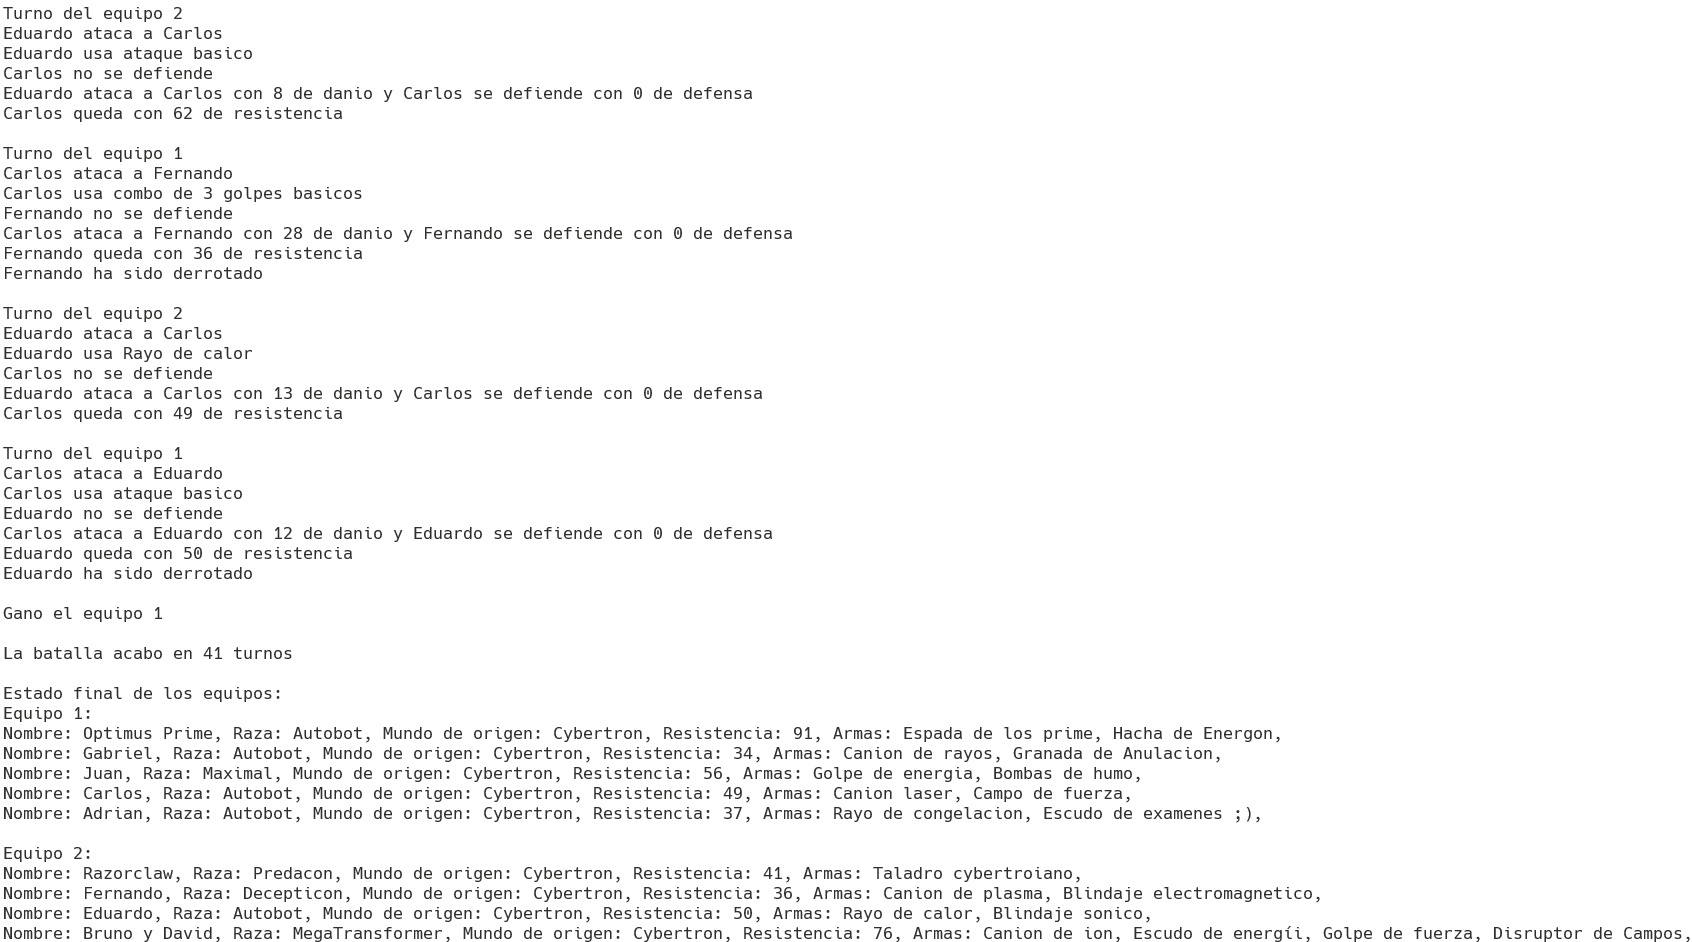
\includegraphics[width = \textwidth, center]{transformers.png}
    \end{figure*}
  \end{enumerate}

  \section*{Referencias}
  Diagrama de clases. Teoria y ejemplos. (2023, 28 marzo). DiagramasUML.com. \url{https://diagramasuml.com/diagrama-de-clases/} \\

  Diagrama de objetos. (2019, 8 diciembre). DiagramasUML.com. \url{https://diagramasuml.com/objetos/} \\

  Introducing EDrawMax 10. (s. f.). Edrawsoft. \url{https://www.edrawsoft.com/es/article/component-diagram-uml.html} \\

  Diagrama de paquetes. (2019, 8 diciembre). DiagramasUML.com. \url{https://diagramasuml.com/paquetes/} \\

  Manzanares, N. A. F. (s. f.). Diagramas de casos de uso | LENGUAJE DE MODELADO UNIFICADO UML. \url{https://unadzsurlab.com/UML/U1/diagramas_de_casos_de_uso.html}
\end{document}